\documentclass[12pt]{article}

\usepackage[a4paper,margin=1in]{geometry}
\usepackage{setspace}
\usepackage{lmodern}
\usepackage[english]{babel}
\usepackage{mathtools,amsthm,amssymb,amsmath}
\numberwithin{equation}{section}
\usepackage{booktabs} % For better-looking tables
\usepackage{dcolumn}  % For aligning decimal points in tables
\usepackage{hyperref}
\usepackage{ marvosym }
\usepackage{eurosym}
\usepackage{bm}
\usepackage{graphicx}
\usepackage[longnamesfirst]{natbib}
\usepackage{float}
\usepackage{longtable}
\usepackage{caption}
\usepackage{listings}
\usepackage{xcolor}

\lstdefinelanguage{SQL}{
    keywords={SELECT, FROM, WHERE, INSERT, INTO, UPDATE, DELETE, CREATE, TABLE, ALTER, DROP, JOIN, ON, AND, OR, NOT, NULL, PRIMARY, KEY},
    keywordstyle=\color{blue}\bfseries,
    comment=[l]{--},
    commentstyle=\color{gray}\ttfamily,
    stringstyle=\color{red},
    morestring=[b]',
    morestring=[b]"
}

\lstdefinelanguage{Python}{
    keywords={def, return, if, elif, else, while, for, in, try, except, finally, with, as, import, from, class, pass, break, continue, and, or, not, is, None, True, False, lambda, yield, global, nonlocal, assert, raise},
    keywordstyle=\color{blue}\bfseries,
    comment=[l]\#,
    commentstyle=\color{gray}\ttfamily,
    stringstyle=\color{red},
    morestring=[b]',
    morestring=[b]"
}

\lstset{
    basicstyle=\ttfamily,
    columns=fullflexible,
    language=SQL,
    frame=single,
    backgroundcolor=\color{gray!10}
}

\setlength{\parindent}{0pt}     % No paragraph indentation
\setlength{\parskip}{1em}       % Add vertical space between paragraphs

\newcommand{\N}[1]{\mathcal{N}\left(#1\right)}
\newcommand{\Z}{\mathbb{Z}}
\DeclareMathOperator*{\argmin}{arg\,min}
\DeclareMathOperator*{\argmax}{arg\,max}
\newcommand{\abs}[1]{\left\vert#1\right\vert}
\newcommand{\given}{\,\middle|\,}
\newcommand{\Bern}[1]{\mathrm{Bern}(#1)}
\newcommand{\Bin}[1]{\mathrm{Bin}(#1)}
\newcommand{\Exp}[1]{\mathrm{Exp}(#1)}
\newcommand{\FS}[1]{\mathrm{FS}(#1)}
\newcommand{\Geo}[1]{\mathrm{Geo}(#1)}
\newcommand{\Norm}[1]{\mathrm{Norm}(#1)}
\newcommand{\Pois}[1]{\mathrm{Pois}(#1)}
\newcommand{\Unif}[1]{\mathrm{Unif}(#1)}
\newcommand{\E}[1]{\,\mathsf{E}\left[#1\right]}
\newcommand{\EE}[2]{\,\mathsf{E}_{#1}\left[#2\right]}
\newcommand{\V}[1]{\,\mathsf{V}\left[#1\right]}
\newcommand{\cov}[1]{\,\mathsf{Cov}\left[#1\right]}
\renewcommand{\d}[1]{\,\textrm{d}#1}
\newcommand{\1}[1]{\,I_{#1}} % indicator
\renewcommand{\P}[1]{\,\mathbb{P}\left\{#1\right\}}
\renewcommand{\cos}[1]{\text{cos}\left[#1\right]}
\newcommand{\fat}[1]{\ThisStyle{\hstretch{1.2}{\ooalign{%
  \kern.46pt$\SavedStyle#1$\cr\kern.33pt$\SavedStyle#1$\cr%
  \kern.2pt$\SavedStyle#1$\cr$\SavedStyle#1$}}}}
\renewcommand{\ln}[1]{\,\mathrm{ln}\left[#1\right]}
\newcommand*{\B}[1]{\ifmmode\bm{#1}\else\textbf{#1}\fi}
\pagestyle{empty}

\title{Assessment of an approximation method for TSP path length on road networks}
\author{Koen Stevens}
\date{\today}
\begin{document}
\begin{titlepage}
	\centering
	\vspace*{0.3\textheight}
	{\LARGE\bfseries Assessment of an approximation method for TSP path length on road networks \par}
	\vspace{2cm}
	{\Large Koen Stevens \par}
	\vfill
	{\large \today \par} % or hardcode the date
\end{titlepage}
\clearpage
\thispagestyle{empty}
\vspace*{0.3\textheight}
{\Large Bachelor's Thesis Econometrics \par}
\vspace{1cm}
{\large Supervisor: dr. N.D. van Foreest \par}
\vspace{0.5cm}
{\large Second assessor:  \par}
\clearpage
\pagenumbering{arabic}
\pagestyle{plain}
\begin{center}
	\LARGE \textbf{Assessment of an approximation method for TSP path length on road networks} \\[1.5ex]
	\large Koen Stevens
\end{center}
\begin{abstract}

\end{abstract}
\section{Introduction}
The Traveling Salesman Problem (TSP) is an important problem in operations research.
It is particularly relevant for last-mile carriers and other logistics companies where efficient
routing directly impacts cost, time and service quality. Since the number of parcels worldwide has
increased between 2013 and 2022 and is expected to keep increasing \citep{statista}, the need for
fast, scalable route planning methods becomes ever more pressing.

The TSP is an NP-hard problem, it is computationally intensive to find the exact solution for
large instances. In many real-world scenarios, the exact optimal routes may not be needed, but
instead a rough, reliable estimate of the optimal route length. For instance, consider a postal delivery company.
This firm may need to assign a certain amount of deliveries or a certain area to each postman.
Reliable estimates for the route length can provide valuable information for making such decisions.

Efficient approximation methods provide a solution for such practical applications where exact
solutions are too computationally intensive to conduct or not feasible due to insufficient data.
These methods aim at approximating the expected optimal total travel time or distance, while using
minimal data and computational effort.

There is extensive research on such approximation methods and how they perform in the Euclidean
plane.
Consider $n$ uniformly drawn locations from some area in $\mathbb{R}^2$ with area $A$.
\citet{beardwood1959shortest} prove the relation:
\begin{align}
	L \to \beta \sqrt{nA}, \quad \text{as } n \to \infty
	\label{eq:beardwood}
\end{align}
as an estimation for the length of the shortest TSP path measured by Euclidean distance through
these random locations, where $\beta$ is some proportionality constant. This formula is a very
elegant result, and it requires very little data. However, its assumptions,
uniform random locations and euclidean space differ from real-world applications, which are defined
by complex geographic features, such as road networks.

This research investigates how well this approximation method performs when considering real road
networks. Using OpenStreetMap \citep{openstreetmap} data, TSP instances are simulated in a wide variety of different urban areas
in the Netherlands, then solve these for the actual shortest paths using the Lin–Kernighan heuristic
\citep{lin1973effective}.
Then, the $\beta$ from equation \ref{eq:beardwood} is estimated and the performance of this
formula is analyzed. Additionally, the results for $\beta$ and the performance across the selected
areas is compared. 

The core contribution of this research is the performance of the Beardwood formula is analyzed when: 
\begin{enumerate}
  \item relaxing the assumption of uniformly drawn locations. In this research,
	the locations are drawn from the set of postcodes in the area in question.
  \item applied to realistically sized real-world parts of cities and villages in the Netherlands.
\end{enumerate}
The analysis can easily be extended to any type of area in any part of the world, one would only
have to download the OpenStreetMap \citep{openstreetmap} for another part of the world and add the names of the areas
to apply it to. The source code of this project is available on 
\href{https://github.com/koen1859/Scriptie}{GitHub}.

In section 2 a deep dive in the context and previous research in this field is provided.
In section 3 the experimental design is documented.
\section{Literature Review}
In this section the existing literature on the Beardwood formula and some applications,
and on the Lin-Kernighan heuristic and its implementations is reviewed.
\subsection{Applications of the Beardwood formula}
This research concerns the performance of formula \ref{eq:beardwood} for reasonable amounts of
locations a delivery person can visit in a workday, say $10\leq n\leq90$.
\citet{lei2015dynamic} estimates the values of $\beta$ for a selection of values for $n$.
In their research, the points were generated uniformly and the $L_2$ distance metric was used.
Table \ref{tab:beta-values} lists the results.
\begin{table}[H]
	\centering
	\caption{Empirical estimates of $\beta$ as a function of $n$, $20 \leq n \leq 90$\\
		\citep{lei2015dynamic}}
	\label{tab:beta-values}
	\begin{tabular}{cc}
		\toprule
		$n$ & $\beta(n)$ \\
		\midrule
		20  & 0.8584265  \\
		30  & 0.8269698  \\
		40  & 0.8129900  \\
		50  & 0.7994125  \\
		60  & 0.7908632  \\
		70  & 0.7817751  \\
		80  & 0.7775367  \\
		90  & 0.7773827  \\
		\bottomrule
	\end{tabular}
\end{table}
\citet{figliozzi2008planning} is the first research to apply approximation formulas to real-world
instances of TSPs (and VRPs (Vehicle Routing Problems)). An extension of formula
\ref{eq:beardwood} that works for VRPs is assessed in a real-world setting. It is found that this
model has an $R^2$ of 0.99 and MAPE (Mean Absolute Prediction Error) of 4.2\%. This prediction error
is slightly higher than when it is applied to a setting where Euclidean distances are considered (3.0\%),
but the formula still performs well \citep{figliozzi2008planning}.

\citet{merchan2019empirical} use circuity factors to measure the relative detour incurred for
traveling in a road network, compared to the Euclidean distance. This circuity factor is defined
as, where $p$ and $q$ are locations:
\begin{align}
	c = \frac{d_{c}(p,q)}{d_{L_{2}}(p,q)}
	\label{eq:circuity}
\end{align}
By construction, $c$ is greater or equal to 1, a value closer to 1 indicates a more efficient network. Then, $\beta_c$
is estimated by $\beta_c=c\beta$. This value $c$, is estimated for three different areas in
São Paulo, for which the results are listed in table \ref{tab:beta-merchan}. These values indicate
real travel distances are on average 2.76 times longer in area 1 compared to the $L_2$ metric.
These values were obtained by uniformly generating $n$ locations (for $n$ ranging from 3 to 250),
computing near-optimal tour lengths under the Euclidean metric, and solving for $\beta$, then
scaling by the empirical circuity factor.
\begin{table}[htbp]
	\centering
	\caption{Estimates of the circuity factor $c$ and its corresponding $\beta_c$ \citep{merchan2019empirical}}
	\label{tab:beta-merchan}
	\begin{tabular}{lccc}
		\toprule
		          & Area 1 & Area 2 & Area 3 \\
		\midrule
		$c$       & 2.76   & 2.34   & 1.82   \\
		$\beta_c$ & 2.48   & 2.10   & 1.64   \\
		\bottomrule
	\end{tabular}
\end{table}
It is important to note, however, that the assumptions in this study may limit the generality of
the findings. In particular, the use of uniformly distributed locations does not accurately reflect
the spatial distribution of delivery points in real urban environments, where locations tend to
cluster in residential, commercial, or industrial zones. Additionally, within small urban areas,
high-rise buildings and single-family homes may coexist in the same neighborhoods, further
challenging the assumption of uniformly distributed delivery points.
Furthermore, the circuity factor $c$ can
vary significantly within a single city, depending on local street patterns, infrastructure, and
topography. These variations suggest that a fixed circuity factor may oversimplify the complexity
of real-world delivery contexts, especially when applied to smaller sub-regions or neighborhoods.
\subsection{Lin-Kernighan Heuristic}
To be able to efficiently solve many TSPs, to find a good estimate for $\beta$, a fast and reliable
solution algorithm is needed. The Lin-Kernighan \citep{lin1973effective} heuristic provides outcome,
it is generally considered to be one of the most effective methods of generating (near) optimal
solutions for the TSP.
In this research a modified implementation of the heuristic is used \citep{helsgaun2000effective}.
The run times of both heuristics increase by approximately $n^{2.2}$, but the modified heuristic is
much more effective. It is able to find optimal solutions to large instances in reasonable times
\citep{helsgaun2000effective}.

\underbar{PARAGRAPH ABOUT HOW THE HEURISTIC WORKS}
\section{Experimental design}
In this section, a detailed explanation of the methodology is provided. This includes the 
characteristics of the data used, how this data is processed, as well as the approach taken to 
generate and solve TSP instances.
\subsection{Data}
In order to model the complex nature of real road networks, data from OpenStreetMap \citep{openstreetmap} is used. 
OpenStreetMap is an open-source project that provides geographic data, including accurate and 
detailed information about roads, buildings and natural features around the world. The data is 
continuously maintained and updated by a large community of users, making it a valuable resource 
for this research.

This data can be downloaded from Geofabrik, and then exported to a \url{PostgreSQL} database using
\url{osm2pgsql} \citep{osm2pgsql}, in order to be able to efficiently use the data with \url{Python}. 
For this analysis, the database has three interesting tables: 
\url{planet_osm_polygon}, \url{planet_osm_nodes} and \url{planet_osm_ways}.

A large number of neighborhoods multiple towns and villages in the Netherlands have a polygon 
defined in the data. In OpenStreetMap a polygon is a closed shape formed by a set of geographic coordinates 
(\url{nodes}) that are connected by lines (\url{ways}). These objects can be used to define boundaries of
geographic areas, such as lakes, parks, nature reserves and parts of cities and villages. In this
research the polygons are used to filter the buildings and roads only in a certain area efficiently.
These polygons are stored in \url{planet_osm_polygon}.

In the database, the roads are defined as \url{ways}. These ways have three
attributes: \url{id}, \url{nodes} and \url{tags}. The attribute \url{nodes} contains an ordered list
of the nodes that this road contains of.
In the \url{tags}, a large amount of 
information about the way is stored, for instance whether it is a 
one-way road, or the type of road that it is, i.e. primary, or trunk.
The information about the roads that are needed for this analysis is the
road id, the ids of the nodes the road consists of, the coordinates
(Latitude, Longitude) of these nodes, and whether the road is a one-way
road.

The buildings are stored as \url{nodes}. In this table (\url{planet_osm_nodes}),
a large amount of other objects are stored as well. For this analysis,
the potential delivery locations need to be extracted. Some of these 
nodes have a postcode defined, which can be used to extract all buildings
that a potential delivery could take place. This way, for example a little shed in 
someones backyard is also filtered out, since this does not have its own 
postcode. For this research only the node id and the coordinates are
needed.

\subsection{Data processing}
In listing \ref{lst:sql-roads} (Appendix), the query that is used to extract
all roads in an area is listed. This query is used inside an \url{f-string}
in \url{Python}, to be able to loop over the different areas and extract
the roads from it. Note that a buffer of a few meters around the neighborhood
is used for the filtering, since otherwise this results in edge cases,
where a road is ever so slightly more to the outside of the area than the boundary,
and it would get left out. \url{ST_Intersects} is used to extract all roads
that are at least partly inside or on the boundary. A similar query is used 
to extract the nodes, but this is easier since for a building which is only
defined by a single node, it is not needed to define a new geometry object.

One of the predictors of the TSP path length, is the area of the neighborhood
the locations are drawn from. The OSM data provides the area of the polygons,
but this value can not be used to predict TSP path length effectively.
This value is a heavy overestimation of the correct value for $A$.
In many cases, there are parts of the neighborhood that do not contain
any buildings, for instance when there is a park in the neighborhood. To
account for this, the value for $A$ that is used, is the area of the convex
hull around all buildings, which is calculated using the \url{shapely}
module in \url{Python}. As an example visualization, figure \ref{fig:binnenstad_quarter} displays
how the quarter for the inner city of Groningen is defined in OpenStreetMap. Using the area of this
entire quarter would be an overestimation. A significant portion of this area is the canal and outer
road around the inner city. There are many examples of quarters where this overestimation is even
more significant than this.
\begin{figure}[H]
  \caption{The OpenStreetMap quarter for the inner city of Groningen (Binnenstad). \citep{openstreetmap}}
  \label{fig:binnenstad_quarter}
  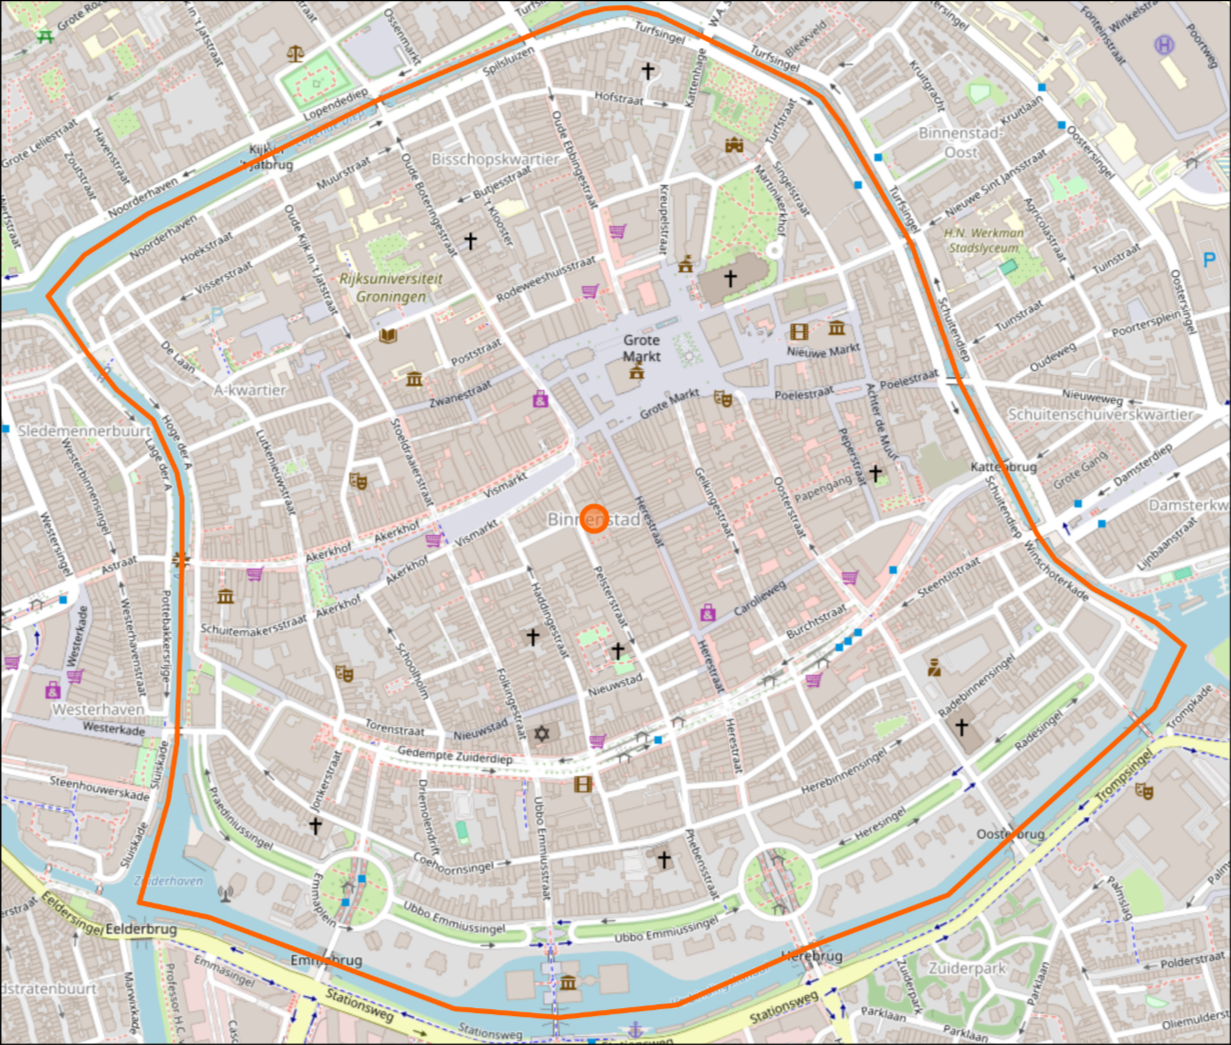
\includegraphics[width=\textwidth]{Pictures/Binnenstad_quarter.png}
\end{figure}
Using the geographic information of the roads and buildings, a graph
is constructed, using the \url{igraph} module in \url{Python}. This graph
connects all buildings to each other over the road network. First, using the information about the 
roads and buildings the sets of nodes and edges need to be defined. An edge is a line that connects
two edges to each other. Extracting the edges that connect the road network is straightforward,
since all roads already have an ordered list of nodes defined. The subsequent nodes simply need to
be stored as pairs, and all edges are defined.

When the road network is defined as a set of nodes and edges, the next step is to connect the buildings
to the road network. This needs to be done manually, since no data is stored in OpenStreetMap 
about to which road the buildings belong. This algorithm needs to be very efficient, since many 
buildings are added in each area. An R-tree can be used to accomplish this efficiency.
An R-tree is a dynamic index structure that is able to retrieve data items quickly according to 
their spatial locations \citep{guttman1984r}. Listing \ref{lst:python-edges} displays the algorithm
used to make the edges that connect the buildings to the road network. For each building node,
the closest point on the closest road is found, using the shapely implementation of the R-tree,
\url{STRtree}. Then, if this point is not an already existing node, a new virtual node is added,
which splits this existing edge in two parts. The road is reconnected with the new node in between.
Finally, the building is connected to this new node.

In order to find the shortest path in terms of real distance, and to calculate the length of the 
TSP path, a 'weight' needs to be added. This weight represents the length of this edge in meters.
The equirectangular approximation is used to calculate these weights. This approximation is very
efficient, but only works when the points the distance is calculated between is small enough such
that the rounding of the earth does not have a significant effect on the true distance.
The nodes are all close enough together, so the effect of the 
rounding of earth's surface is negligible. Let $A$ and $B$ be two nodes,
and $(x_A,y_A)$, $(x_B),y_B)$ be their coordinates, in \url{radians}. Let $R=6,371,000$ meters, 
Earth's radius. Then the distance between these nodes (the weight of the edge connecting them),
using the equirectangular approximation is:
\begin{align}
  \label{eq:equirectangluar_approx}
  d(A,B)	&=R\sqrt{x^2+y^2},\\
  \text{where }x&=(x_B-x_A)\cos{\frac{y_A+y_B}{2}},\\
  \text{and }y	&=y_B-y_A.
\end{align}

Using the \url{folium} module in \url{Python}, such a graph can be projected back onto the world map.
One of such visualizations is provided in figure \ref{fig:overtoomse_sluis}. All maps like this one,
for the areas in this analysis can be viewed and interacted with via this 
\href{https://koenstevens.nl/wp-content/uploads/maps/}{\url{webpage}}.
\begin{figure}[H]
  \caption{Visualization of the graph, for the Overtoomse Sluis quarter in Amsterdam.}
  \label{fig:overtoomse_sluis}
  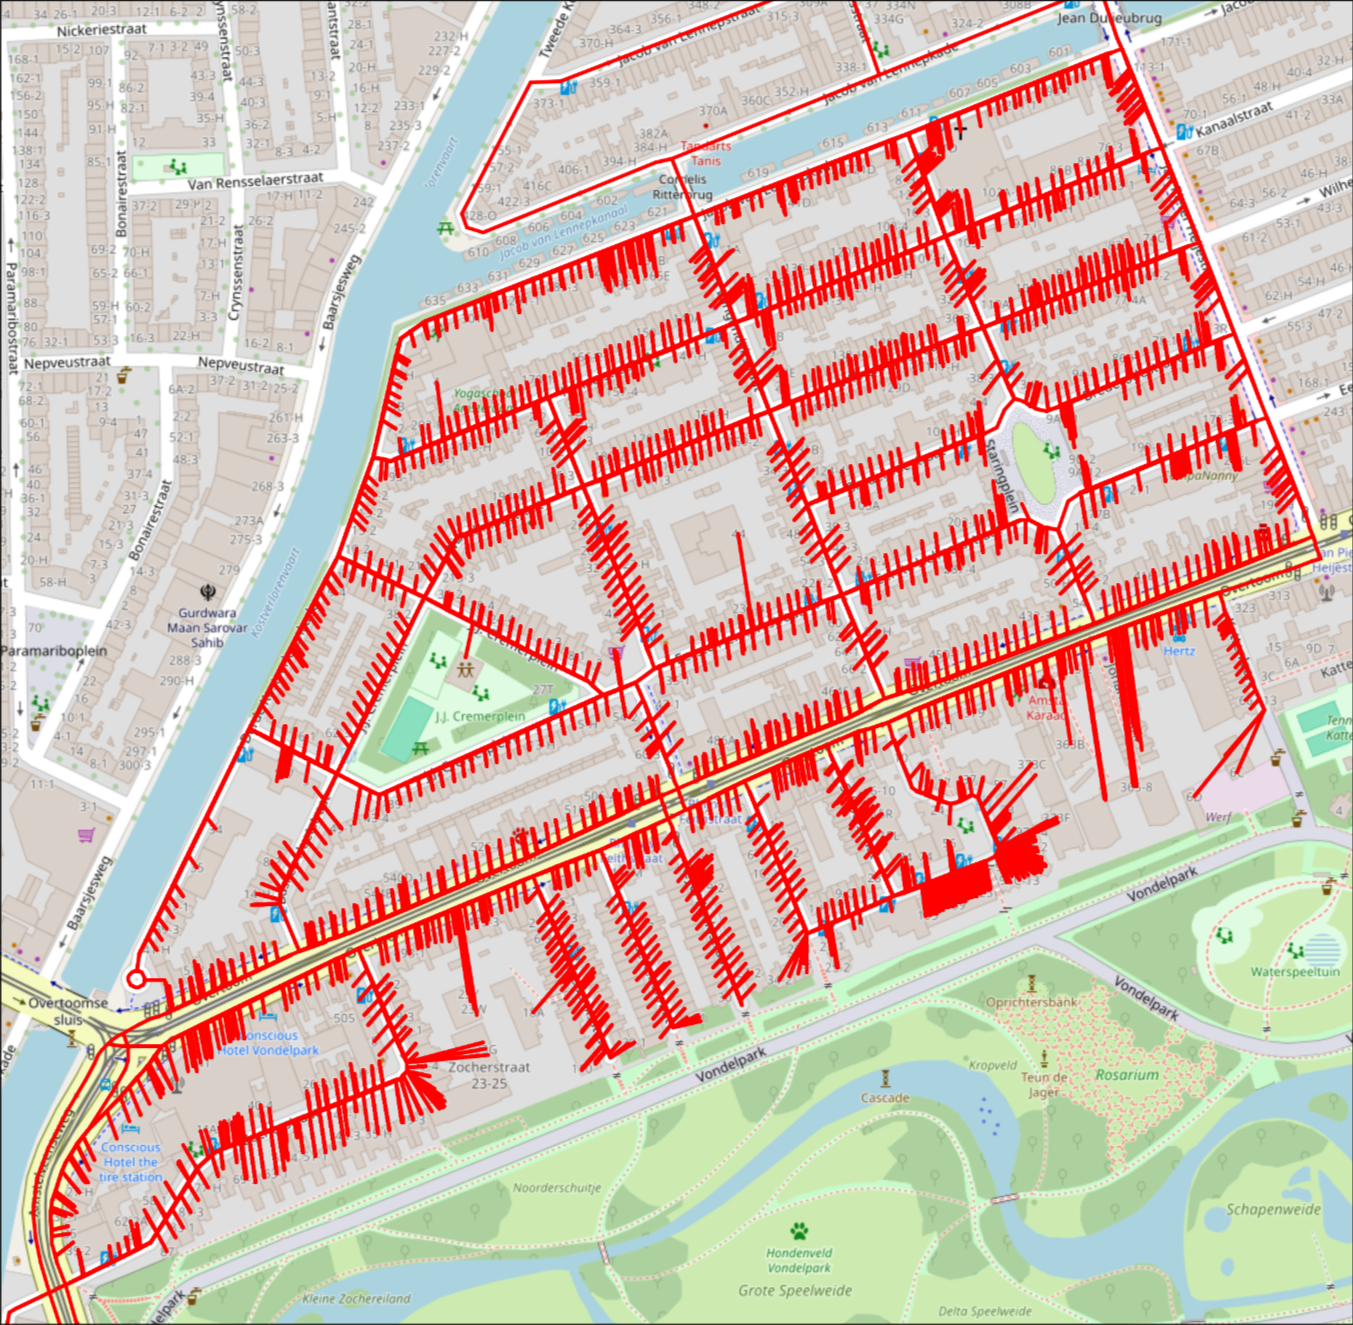
\includegraphics[width=\textwidth]{Pictures/Overtoomse_Sluis_roads.png}
\end{figure}
\subsection{Generating and solving TSPs}
First, a uniform random sample is taken out of the list of buildings, of size\\
$n\in\{20, 22, \cdots, 86, 88\}$. For each $n$, 100 samples are taken. Then, using the very neat
builtin \url{igraph} function, \url{shortest_paths_dijkstra}, a distance matrix can be constructed
over the graph in a very efficient manner. Using the sample of buildings and the corresponding 
distance matrix, three files need to written per instance: a parameter file, a problem file and a 
\url{json} file.

The parameter file contains two lines, in this case: a path to the problem file and a path to the
output tour file. This ensures that LKH solvers the correct TSPs, and saves the solutions in the 
correct locations. The problem file contains the information about the problem, for instance
$n$, and the distance matrix. Using these two inputs LKH can solve the TSPs. However with only these 
two files, the output tour can not be evaluated, since LKH starts indexing the visited locations
from 1, and can not take different location ids as input. The \url{json} file saves a \url{Python}
dictionary that maps these indexes back to the correct node indices, so the output can be read.

Using the \url{multiprocessing} module in \url{Python}, as many TSPs are solved at the same time
as the number of threads in the processor that the project is ran on. LKH writes the solutions,
with their respective path lengths to another file, that can then be read back into \url{Python},
to analyze the results. This process is repeated for a selection of 29 areas in the province of
Groningen and for 52 areas in North Holland.

Again using the \url{folium} module, such a solution path can be visualized on the map. One of such
paths is provided in figure \ref{fig:tsp_stadvdzon}. Only some of these paths are visualized,
in order to check whether it looks like a reasonable solution, but it is not feasible, and it does
not add value to visualize all TSP paths, since there is a total of 
$(29+52)\cdot70\cdot100=567,000$ TSP simulations.
Using the TSP solutions LKH provides and the estimated area of each neighborhood, formula 
\ref{eq:beardwood} can be estimated.
\begin{figure}[H]
  \caption{Visualization of a solved TSP path with 22 locations, for the Stad van de Zon quarter in 
  Heerhugowaard (North Holland).}
  \label{fig:tsp_stadvdzon}
  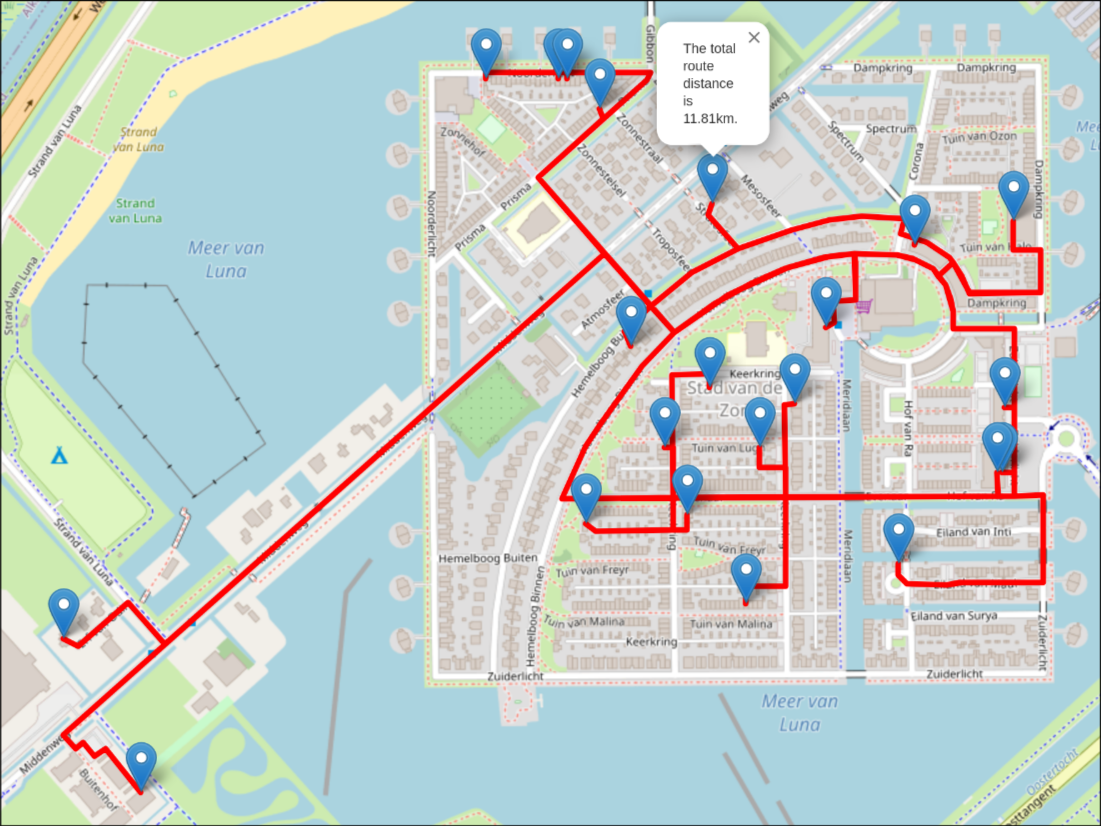
\includegraphics[width=\textwidth]{Pictures/TSP_22_Stad_van_de_Zon.png}
\end{figure}
\section{Results}
\section{Discussion}
\section{Conclusion}
\bibliography{literature}
\bibliographystyle{rug-econometrics}
\section{Appendix}
\subsection{Listings}
\begin{lstlisting}[caption={The query to extract roads inside a neighborhood.}, label={lst:sql-roads}]
-- First, get the neighborhood polygon, in the coordinate format we need.
WITH neighborhood AS (
    SELECT ST_Transform(way, 4326) AS geom
    FROM planet_osm_polygon
    WHERE place = 'quarter'
      AND name = '{neighborhood}'
),
-- Then, define the road geometries in a way that we can filter based 
-- on whether they are inside the neighborhood.
road_geometries AS (
    SELECT
	w.id AS road_id,
	w.nodes AS node_ids,
	w.tags->>'oneway' AS oneway,
	ST_MakeLine(ARRAY(
	    SELECT ST_SetSRID(
		ST_MakePoint(n.lon / 1e7, n.lat / 1e7), 4326
		)
	    FROM unnest(w.nodes) WITH ORDINALITY AS u(node_id, ordinality)
	    JOIN planet_osm_nodes n ON n.id = u.node_id
	    ORDER BY u.ordinality
	)) AS road_geom
    FROM planet_osm_ways w
    -- Also filter based on the road type.
    WHERE w.tags->>'highway' IN (
	'trunk', 'rest_area', 'service', 'secondary_link',
	'services', 'tertiary', 'primary', 'secondary',
	'tertiary_link', 'road', 'motorway', 'motorway_link', 
	'corridor', 'primary_link', 'residential', 'trunk_link', 
	'living_street', 'unclassified', 'proposed'
    )
),
-- Filter on whether the roads are at least partly in the neighborhood.
filtered_roads AS (
    SELECT rg.*
    FROM road_geometries rg, neighborhood nb
    WHERE
	ST_Intersects(rg.road_geom, ST_Buffer(nb.geom, 0.0001))
)
-- Select the attributes that are needed.
SELECT
    fr.road_id,
    array_agg(n.id ORDER BY u.ordinality) AS node_ids,
    array_agg(n.lat / 1e7) AS node_lats,
    array_agg(n.lon / 1e7) AS node_lons,
    fr.oneway
FROM filtered_roads fr
JOIN planet_osm_ways w ON fr.road_id = w.id
JOIN LATERAL unnest(w.nodes) 
    WITH ORDINALITY 
    AS u(node_id, ordinality) 
    ON true
JOIN planet_osm_nodes n ON n.id = u.node_id
GROUP BY fr.road_id, fr.oneway;
\end{lstlisting}
\begin{lstlisting}[language=Python, caption={The algorithm to extract the edges to connect the buildings to the road network}, label={lst:python-edges}]
tree = STRtree(road_segments)  # make a tree of the road network

# Counter to add new nodes to connect buildings to road network correctly
new_node_idx = 0
for building_id, building_coords in buildings.items():
    building_point = Point(building_coords)

    # find the nearest edge
    nearest_segment_idx = tree.nearest(building_point)  
    start_node, end_node, oneway = segment_info[nearest_segment_idx]

    # Project the building onto this nearest edge
    nearest_segment = road_segments[nearest_segment_idx]
    projected_point = nearest_segment.interpolate(
	nearest_segment.project(building_point)
    )

    # If the projected point is one of the segments end points, use this
    if projected_point.equals(Point(nodes[start_node])):
	connect_to = start_node
    elif projected_point.equals(Point(nodes[end_node])):
	connect_to = end_node
    # else, we need to create a virtual node
    else:
	virtual_node_id = f"virtual_{new_node_idx}"
	nodes[virtual_node_id] = (projected_point.x, projected_point.y)
	new_node_idx += 1

	# We split the road segment and add the virtual node
	edges.append((start_node, virtual_node_id))
	weights.append(
	  distance(nodes[start_node], nodes[virtual_node_id])
	  )
	edges.append((virtual_node_id, end_node))
	weights.append(
	  distance(nodes[virtual_node_id], nodes[end_node])
	  )

	if oneway != "yes":  # if not one-way, add reverse
	    edges.append((virtual_node_id, start_node))
	    weights.append(
	      distance(nodes[virtual_node_id], nodes[start_node])
	      )
	    edges.append((end_node, virtual_node_id))
	    weights.append(
	    distance(nodes[end_node], nodes[virtual_node_id])
	    )

	# And we need to connect the building to the newly created node
	connect_to = virtual_node_id

    # Finally, we make the connections
    edges.append((str(building_id), connect_to))
    weights.append(distance(building_coords, nodes[connect_to]))
    edges.append((connect_to, str(building_id)))
    weights.append(distance(nodes[connect_to], building_coords))
\end{lstlisting}
\subsection{Tables}
\begin{longtable}{llcc}
\caption{Empirical estimates for $\beta$ in selected neighborhoods.} \label{tab:results}\\
\hline
Province & Neighborhood & $\beta$ & MAE \\
\hline
\endfirsthead
\hline
Province & Neighborhood & $\beta$ & MAE \\
\hline
\endhead
groningen & Hortusbuurt & 2.2049 & 0.0701 \\
groningen & Binnenstad & 2.0410 & 0.0734 \\
groningen & Oosterpoort & 2.0627 & 0.0604 \\
groningen & Rivierenbuurt & 1.7826 & 0.0497 \\
groningen & De Wijert & 1.7755 & 0.0638 \\
groningen & Oosterparkwijk & 1.7838 & 0.0516 \\
groningen & De Hoogte & 1.6922 & 0.0587 \\
groningen & Korrewegwijk & 2.0751 & 0.0537 \\
groningen & Schildersbuurt & 2.2203 & 0.0489 \\
groningen & Paddepoel & 1.6792 & 0.0481 \\
groningen & Oranjewijk & 1.9282 & 0.0545 \\
groningen & Tuinwijk & 2.9039 & 0.0469 \\
groningen & Selwerd & 1.5247 & 0.0478 \\
groningen & Vinkhuizen & 1.4803 & 0.0435 \\
groningen & Hoogkerk-zuid & 1.5621 & 0.0590 \\
groningen & Gravenburg & 1.2985 & 0.0853 \\
groningen & De Held & 1.9223 & 0.0409 \\
groningen & Reitdiep & 1.6478 & 0.0530 \\
groningen & Hoornse Meer & 1.5935 & 0.0447 \\
groningen & Corpus den Hoorn & 1.6088 & 0.0508 \\
groningen & Eemspoort & 1.7165 & 0.0448 \\
groningen & Euvelgunne & 1.9353 & 0.1067 \\
groningen & Driebond & 1.9220 & 0.0599 \\
groningen & Winschoterdiep & 1.9630 & 0.0513 \\
groningen & Eemskanaal & 1.7551 & 0.0418 \\
groningen & Helpman & 2.0721 & 0.0618 \\
groningen & Lewenborg & 1.9303 & 0.0521 \\
groningen & Beijum & 1.7897 & 0.0429 \\
groningen & Maarsveld & 1.6844 & 0.0393 \\
noord holland & Schrijverswijk & 1.7493 & 0.0424 \\
noord holland & Stad van de Zon & 1.4790 & 0.1543 \\
noord holland & Stadshart & 1.4533 & 0.0663 \\
noord holland & Jordaan & 1.8471 & 0.0591 \\
noord holland & Slotervaart & 1.7456 & 0.0437 \\
noord holland & IJburg & 1.3349 & 0.0506 \\
noord holland & Oostelijke Eilanden & 1.6866 & 0.0424 \\
noord holland & Oostelijk Havengebied & 1.7129 & 0.0464 \\
noord holland & Frederik Hendrikbuurt & 2.3020 & 0.0582 \\
noord holland & Van Lennepbuurt & 1.7810 & 0.0596 \\
noord holland & Da Costabuurt & 2.4887 & 0.0585 \\
noord holland & Kinkerbuurt & 1.9679 & 0.0585 \\
noord holland & Kersenboogerd & 1.6571 & 0.0526 \\
noord holland & Pax & 2.1825 & 0.0415 \\
noord holland & Graan voor Visch & 2.2300 & 0.0531 \\
noord holland & Vrijschot-Noord & 2.4427 & 0.0556 \\
noord holland & Toolenburg & 1.2971 & 0.0443 \\
noord holland & Floriande & 1.9124 & 0.0485 \\
noord holland & Overbos & 1.7727 & 0.0419 \\
noord holland & Bornholm & 1.8024 & 0.0399 \\
noord holland & Beukenhorst-Oost & 1.7106 & 0.0833 \\
noord holland & De Hoek & 2.5441 & 0.0554 \\
noord holland & West & 2.0281 & 0.0489 \\
noord holland & Zuid & 1.6462 & 0.0527 \\
noord holland & Oost & 1.8809 & 0.0560 \\
noord holland & Noord & 1.6555 & 0.0485 \\
noord holland & De President & 1.5015 & 0.1269 \\
noord holland & Graan voor Visch-Zuid & 1.7029 & 0.0549 \\
noord holland & Zuidwijk & 1.4000 & 0.0406 \\
noord holland & Buitenveldert-West & 1.1975 & 0.0671 \\
noord holland & Buitenveldert & 1.1503 & 0.0710 \\
noord holland & Apollobuurt & 1.7468 & 0.0617 \\
noord holland & Stadionbuurt & 1.5084 & 0.0638 \\
noord holland & Prinses Irenebuurt e.o. & 1.8819 & 0.0428 \\
noord holland & Hoofddorppleinbuurt & 1.6903 & 0.0704 \\
noord holland & Willemspark & 1.9422 & 0.0576 \\
noord holland & Schinkelbuurt & 1.6424 & 0.0814 \\
noord holland & Vondelparkbuurt & 1.2941 & 0.0521 \\
noord holland & Helmersbuurt & 1.8039 & 0.0540 \\
noord holland & Overtoomse Sluis & 1.9497 & 0.0560 \\
noord holland & Museumkwartier & 1.7178 & 0.0597 \\
noord holland & Rivierenbuurt & 1.6822 & 0.0507 \\
noord holland & IJselbuurt & 1.5712 & 0.0496 \\
noord holland & Scheldebuurt & 1.3686 & 0.0565 \\
noord holland & Rijnbuurt & 1.6555 & 0.0510 \\
noord holland & De Baarsjes & 1.7849 & 0.0578 \\
noord holland & Landlust & 1.7685 & 0.0518 \\
noord holland & Staatsliedenbuurt & 1.8338 & 0.0520 \\
noord holland & Spaarndammerbuurt & 2.2421 & 0.0540 \\
noord holland & De Pijp & 2.2745 & 0.0521 \\
noord holland & Grachtengordel & 1.7832 & 0.0561 \\
noord holland & Oud-Zuid & 1.4443 & 0.0577 \\
\hline
\end{longtable}

\end{document}
